\section{Multiprotocol}
\label{chap:multiprot}
In this chapter I will define the multi-protocol networking in IoT technologies.

\autoref{sec:multi:ov} will give a brief overview of the technology.
\autoref{sec:multi:dc} will showcase some configurations and \autoref{sec:multi:imp} will introduce some implementations that are available.

\subsection{Overview}
\label{sec:multi:ov}
As the IoT market continues to evolve and grow, developers need more integrated options for wireless connectivity. (NXP, website) With multiprotocol-enabled wireless solutions reduce design and development costs and open the path for IoT convergence where applications can leverage the best aspects of multiple connectivity standards.

As the current generation of chips on the market, a multiprotocol implementation usually contains some kind of operating system or a simple scheduler to manage concurrency between the protocols.

Within multiprotocol, the industry specifies different types. In a simple switched multiprotocol, the device's bootloader can switch between two or more protocols. This method does not require an operating system, as the switching is not that dynamic. In switched mode, only one protocol can be loaded at any given time during operation. Figure 3 shows the operation of switched mode.

The other main type is concurrent multiprotocol. This mode allows the device to run multiple protocols on a single radio. The primary features of this type of solution are:
Switch between applications
Manage and configure the physical layer
Protocol prioritization
Real-time scheduling

These features usually call for an operating system. Available from the market, manufacturers do not create this operating system from the ground up. Rather they create a specialized Real-Time Operating System (RTOS).

Some manufacturers offer Linux-based solutions as well as embedded OS. With more powerful and capable embedded computers emerging on the market, devices can run more general operating systems such as Linux. These devices have the capacity to run multiple protocols alongside the OS and an additional IP stack as well. Devices suitable for this workload are being used as gateways or translators between protocols in the IoT realm.

\subsection{Device configuration}
\label{sec:multi:dc}
As I have introduces the main protocols in \autoref{chap:wireless}, I have not mentioned what configurations these can be used. All stacks have a clear separation of what each layer does. This creates a possibility of different manufacturers can implement different layers.

Most manufacturers extend beyond their System-on-Chip (SoC) design and allow more interfaces so their network device to improve reusability. Figure 4 shows different approaches used in the market.

The SoC approach provides all stack-functionality and application-layer components within a single chip. With SoC, developers can write the most optimized solutions with the lowest power consumption. But the whole application is constrained to the actual hardware limitations.

In a Network Co-Processor (NCP) approach, the chip only runs the functions necessary for networking. The most common configuration is that the chip communicates with a second device called the "host" processor via either SPI or UART. The host is responsible for the application management.

\begin{figure}
    \centering
    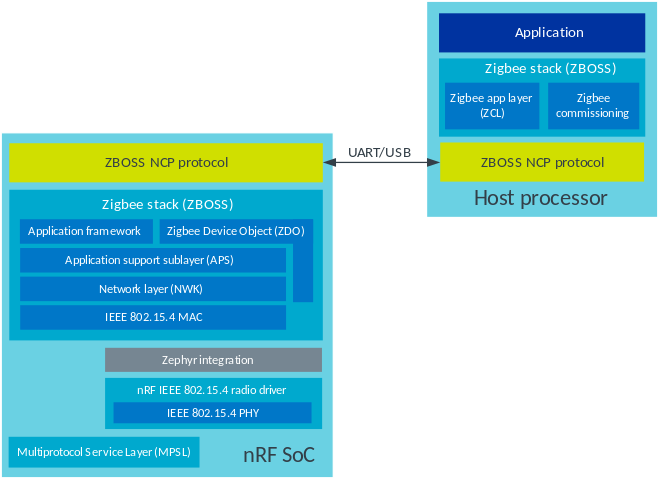
\includegraphics[width=100mm, keepaspectratio]{figures/zigbee_platform_design_ncp-nordicsemi.png}
    \caption{Zigbee Network Co-processor design. Source: \cite{nordic:zigbee}}
    \label{fig:mp:zig-ncp}
\end{figure}

\begin{figure}
    \centering
    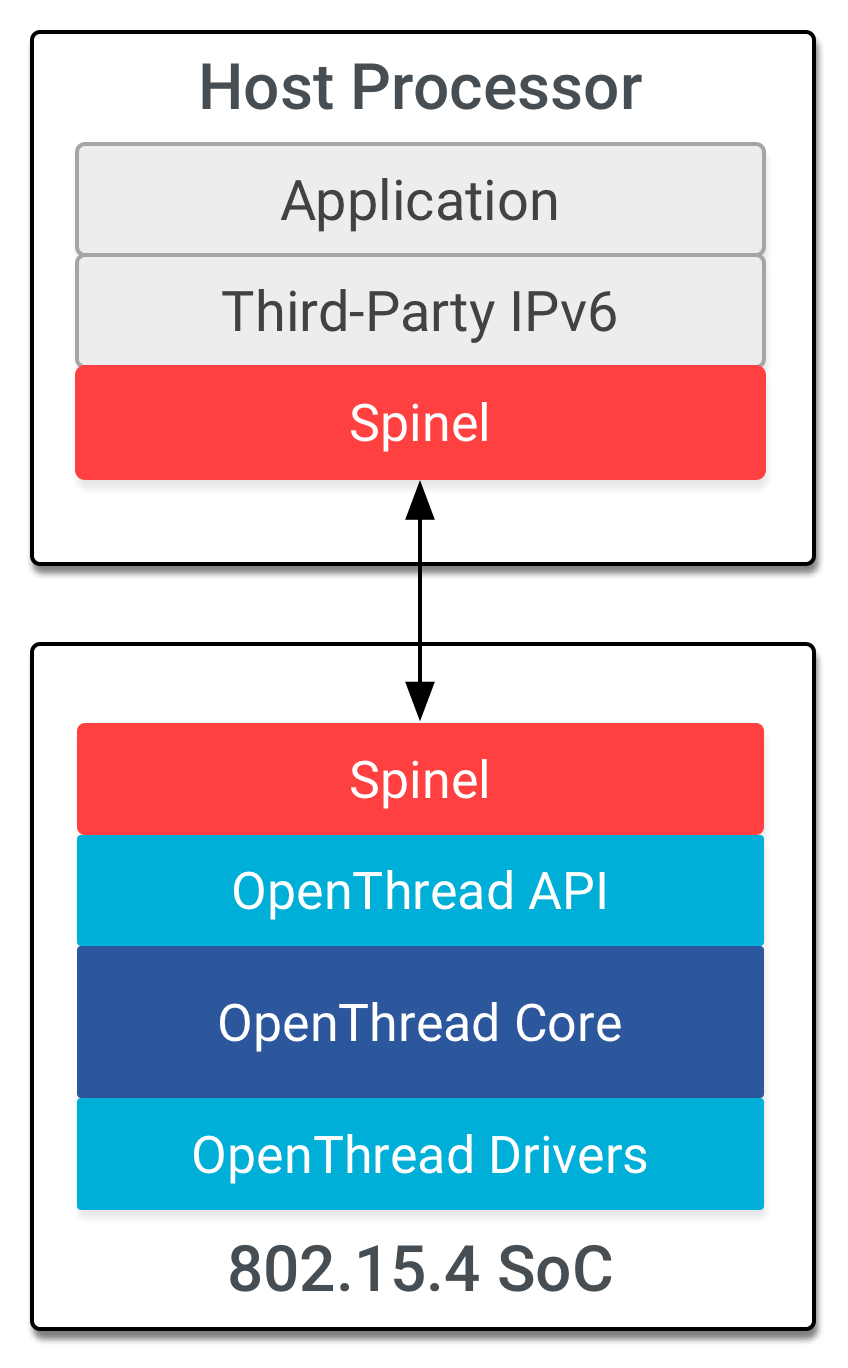
\includegraphics[width=100mm, keepaspectratio]{figures/ot-arch-ncp-vert_2x.png}
    \caption{Thread Network Co-processor design. Source: \cite{thread:platforms}}
    \label{fig:mp:thread-ncp}
\end{figure}

A Radio Co-Processor (RCP) approach is similar to the NCP. The chip only runs the physical layers of the stacks while the host runs the application and network layers. With this architecture integration of multiple protocols that use the same radio band can be better achieved. In BLE, this is achieved with the host-controller-interface (see: \autoref{fig:mp:ble-rcp}). Thread uses the spinnel protocol to control radio devices (see: \autoref{fig:mp:thread-rcp}).

\begin{figure}
    \centering
    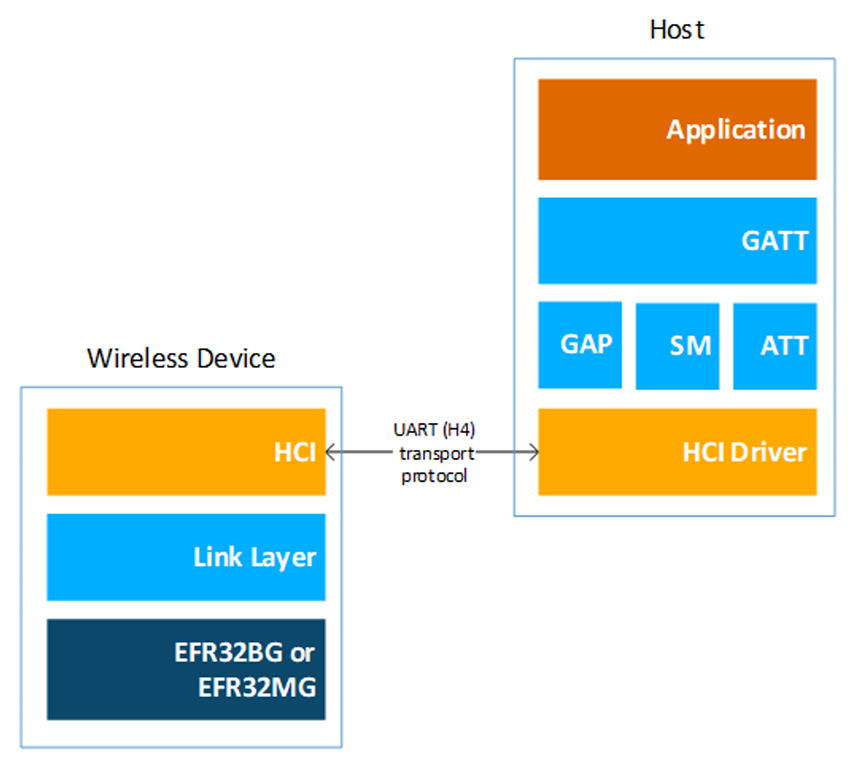
\includegraphics[width=100mm, keepaspectratio]{figures/silabs-ble-rcp-QSG169.png}
    \caption{BLE Radio Co-processor design. Source: \cite{silabs:qsg169}}
    \label{fig:mp:ble-rcp}
\end{figure}
\begin{figure}
    \centering
    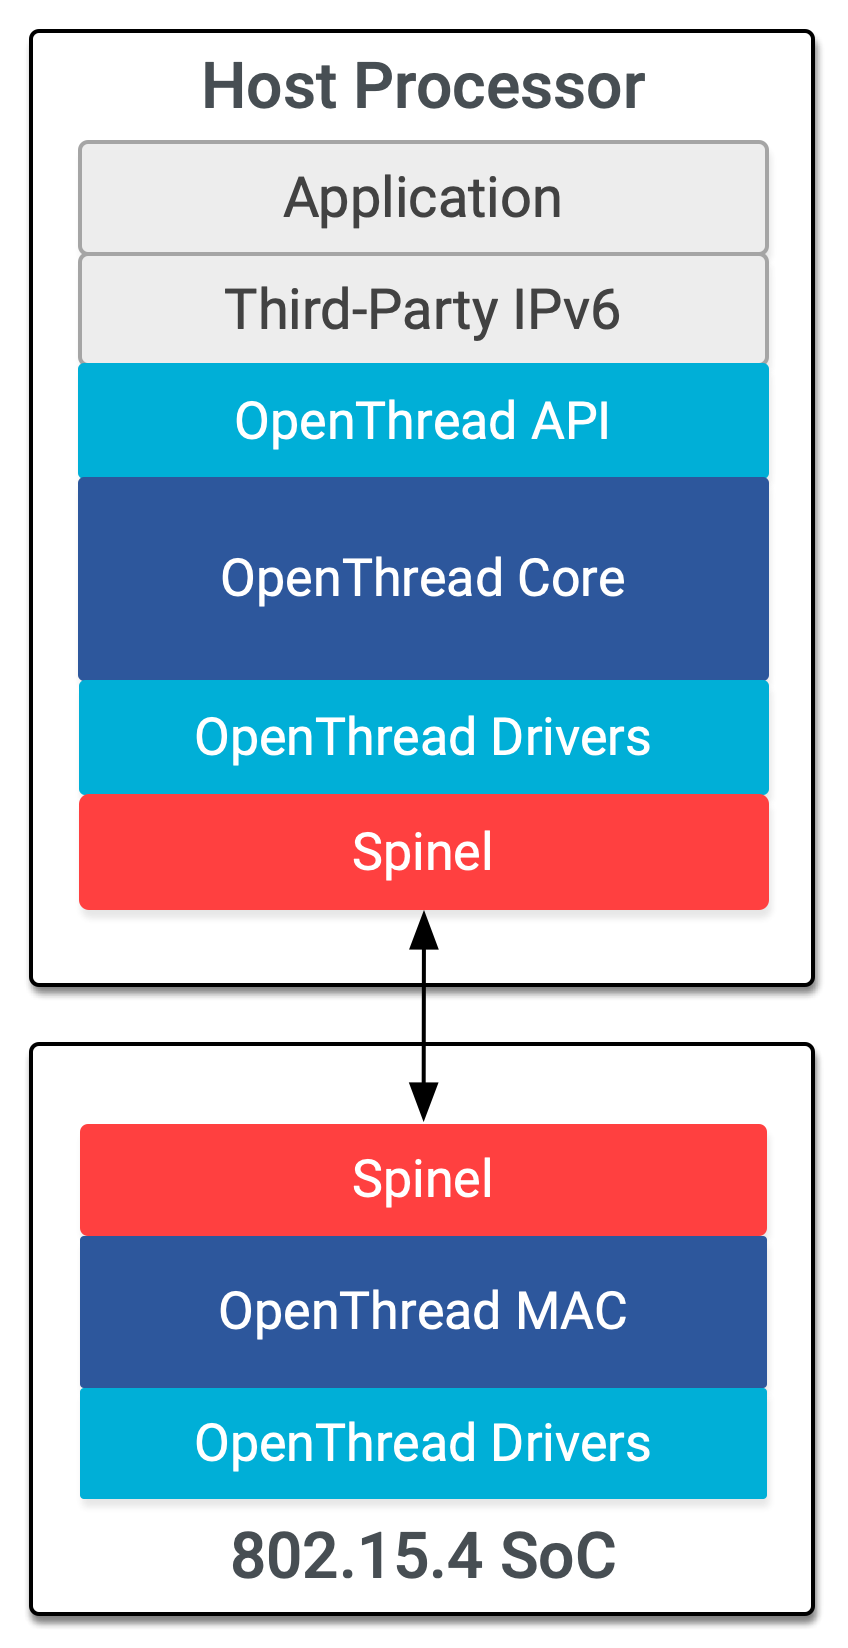
\includegraphics[width=100mm, keepaspectratio]{figures/ot-arch-rcp-vert_2x.png}
    \caption{Thread Radio Co-processor design. Source: \cite{thread:platforms}}
    \label{fig:mp:thread-rcp}
\end{figure}

\subsection{Implementation}
\label{sec:multi:imp}
Based on the Bluetooth, Thread, and Zigbee governing bodies\cite{bt_members:2023, csa_members:2023, thread_members:2023}, four companies are working on and promoting multiprotocol chips: Nordic Semiconductor, NXP Semiconductors, Espressif Systems, and Silicon Laboratories. They all have software development kits (SDKs) that support the development of multiprotocol applications on SoC, NCP, and RCP configuration.

Two distinct approaches could be differentiated between the four companies. Espressif's and NXP's solutions are achieving multiprotocol via having multiple RF transceivers—one for 802.15.4 and another one for Bluetooth. This way, they can use the full range of the 802.15.4 protocol with sub-GHz transmission.

\begin{figure}
    \centering
    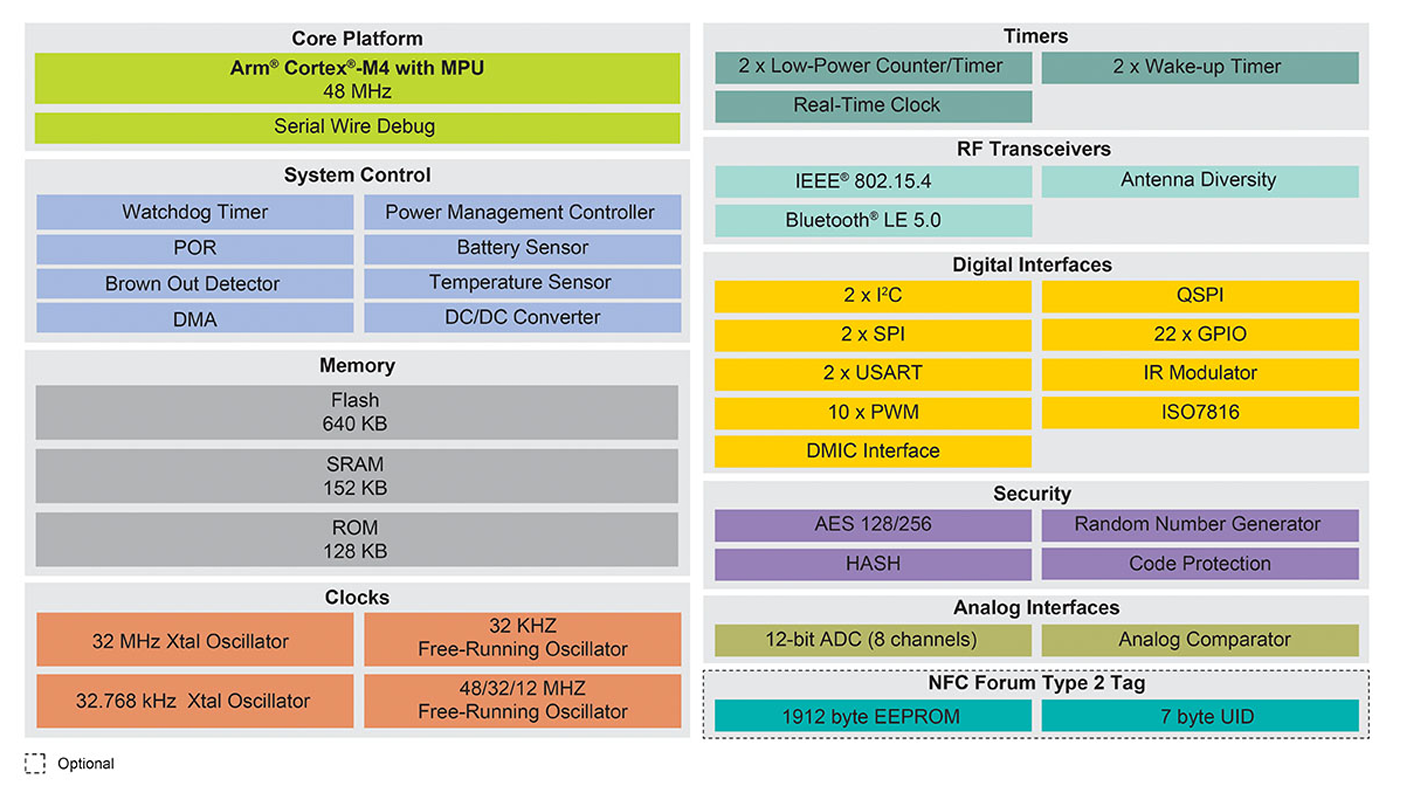
\includegraphics[width=140mm, keepaspectratio]{figures/nxp_k32w061_41-block-dia.png}
    \caption{NXP k32w061 block diagram. Source: \cite{nxp}}
    \label{fig:mp:nxp-dia}
\end{figure}

Silicon Labs and Nordic went with a more packageable approach. Since Bluetooth and 802.15.4 can be operated on the 2,4 GHz frequency range, their solution implements only a single radio transceiver. With this approach, the overall footprint of the device could be smaller. Operating a single radio with multiple stacks could cause issues during communications due to concurrency.

\begin{figure}
    \centering
    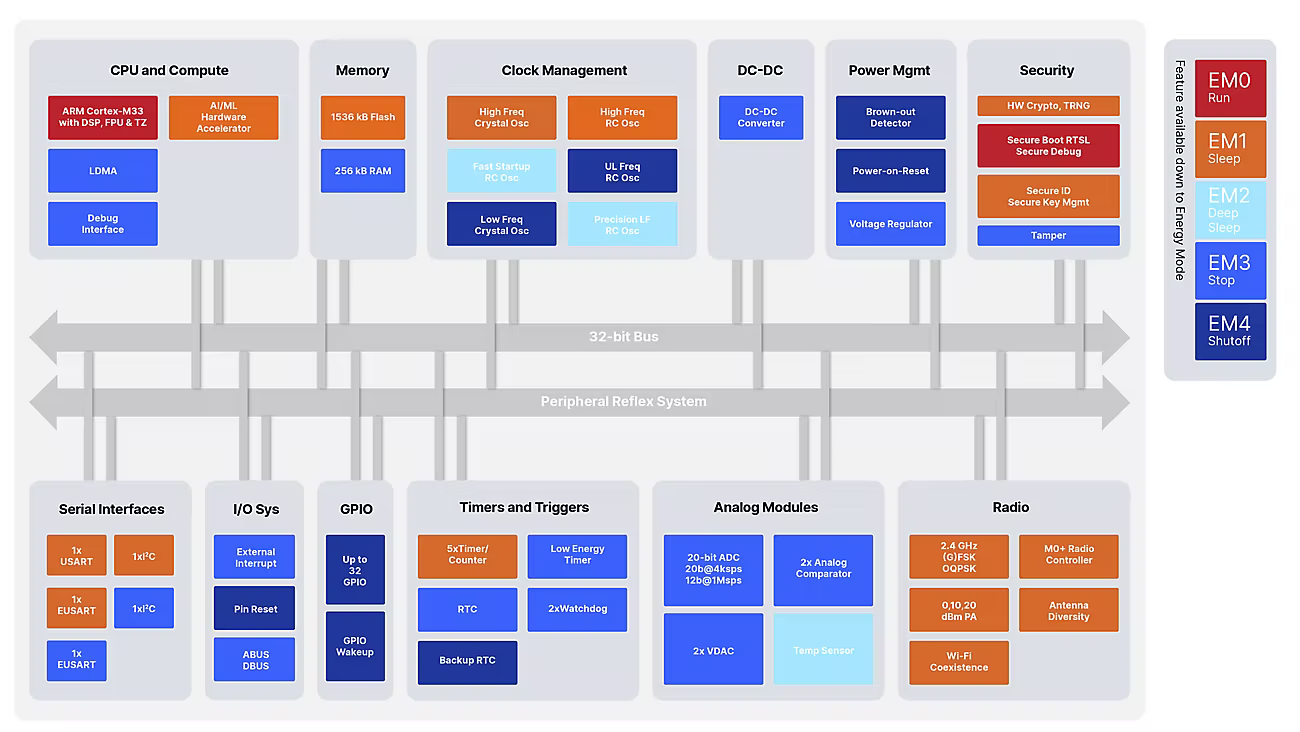
\includegraphics[width=120mm, keepaspectratio]{figures/silabs_xg24-block-diagram.png}
    \caption{Silabs xg24 block diagram. Source: \cite{mg24}}
    \label{fig:mp:silabs-dia}
\end{figure}

\begin{figure}
    \centering
    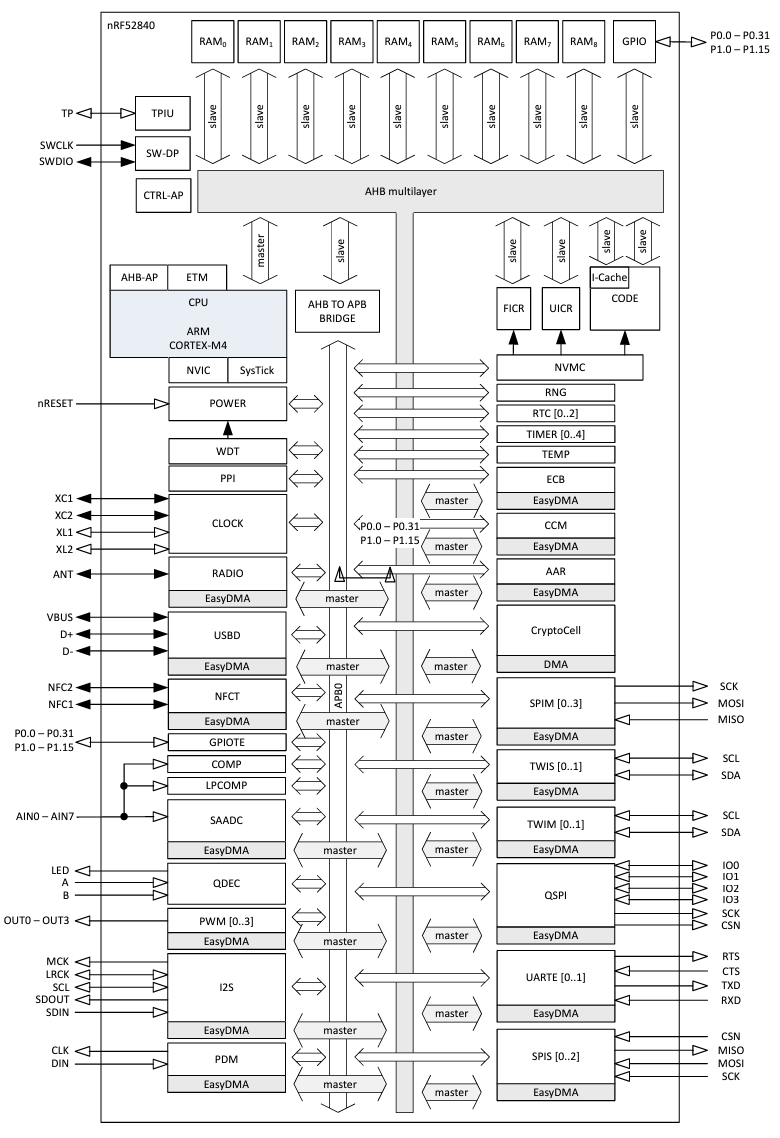
\includegraphics[width=100mm, keepaspectratio]{figures/nordic_nRF52840-block_dia.png}
    \caption{Nordic Semi nRF52840 block diagram. Source: \cite{nordic_semi}}
    \label{fig:mp:nordic-dia}
\end{figure}

All companies mentioned above implement solutions based on an RTOS-flavour operating system for SoC applications and support Linux-based host operating systems for NCP and RCP use cases.